\documentclass[11pt,a4paper]{report}
\usepackage[a4paper,left=20mm,right=20mm,top=25mm,bottom=20mm]{geometry}
\usepackage{amsfonts}
\usepackage{xcolor}
\usepackage{graphicx}
\graphicspath{{./images/}}
\usepackage{csquotes}
\usepackage{hyperref}
\usepackage{listings}
\usepackage{geometry}
\usepackage{float}

\hypersetup{
    colorlinks=true,
    urlcolor=darkgray,
	linkcolor=black
}

\title{\huge{\textbf{Data Mining Project Report}}}
\author{Funaioli Francesca\\
Karoui Hamza\\
Mitola Francesco\\
Vezzuto Samuele\\
}

\begin{document}

\makeatletter
\begin{titlepage}
	\begin{center}
		
\includegraphics[width=0.4\linewidth]{unipi}\\[4ex]
		{\huge \bfseries  \@title }\\[2ex]
		{\Large A.Y. 2023/2024 }\\[6ex]
		{\large  \@author}
	\end{center}
\end{titlepage}
\makeatother

\tableofcontents

\chapter{Data Understanding}

The data understanding phase aims to prepare data for the following data mining tasks and to gain informations on the general properties of our data.
This phase of data analysis is focused on an identification of missing values, outliers, duplicates and distribution analysis.
The three csv files, \texttt{incidents.csv}, \texttt{povertyByStateYear.csv} and \texttt{year\_state\_district\_house.csv} were imported and analyzed separately.
The first preliminary checks comprised looking for null values and checking the data types of the attributes, before a more in depth analysis of each column of each dataset.
By computing the statistics of the numerical values of each dataset, we noticed a wrong value in attribute \textit{participant\_age\_1} (values of 311).
We also found out that some of the columns considered contained non-numerical values, as they were not displayed.
The value of 0 for attribute \textit{participant\_age\_1} occurs when there are infants involved and therefore it is not to be considered a wrong value.
In a similar way, \textit{n\_participants} has value 0 if the incident had no victims or no shots where fired, but also in records with most of the attributes set to null.

\subsection{Incidents}

\subsubsection{Date}

Each \textit{date} value was converted to a datetime object, after checking that there where no null or NaT values.
The plot in Figure \ref{incidents_per_year}, representing the number of incidents per year, shows an increasing trend in the number of crimes over the years.
It also shows a lack of records related to years 2013 and 2018: there are only 253 incidents happened in 2013, hence they will be removed during data preparation.
As for the year 2018, there is only data relating to the first three months of the year in the dataset, so year 2018 will be analyzed on its own.

\begin{figure}[h]
	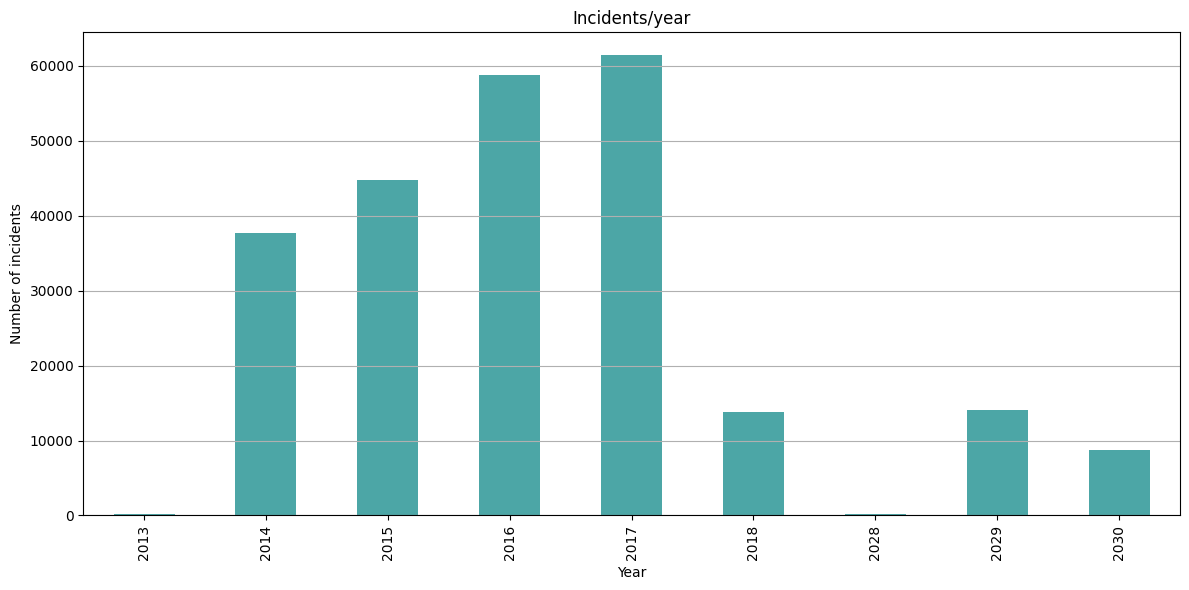
\includegraphics[width=0.8\textwidth]{incidents_per_year}
	\centering
	\caption{Number of incidents per year.}
	\label{incidents_per_year}
\end{figure}

\subsubsection{Geographical information}

The \textit{state} attribute contains no null values and it has 51 unique values: the 50 states of the United States and the District of Columbia, which we will consider as a special state.
Figure \ref{incidents_per_state} shows the number of incidents recorded in each state in decreasing order.

\begin{figure}[h]
	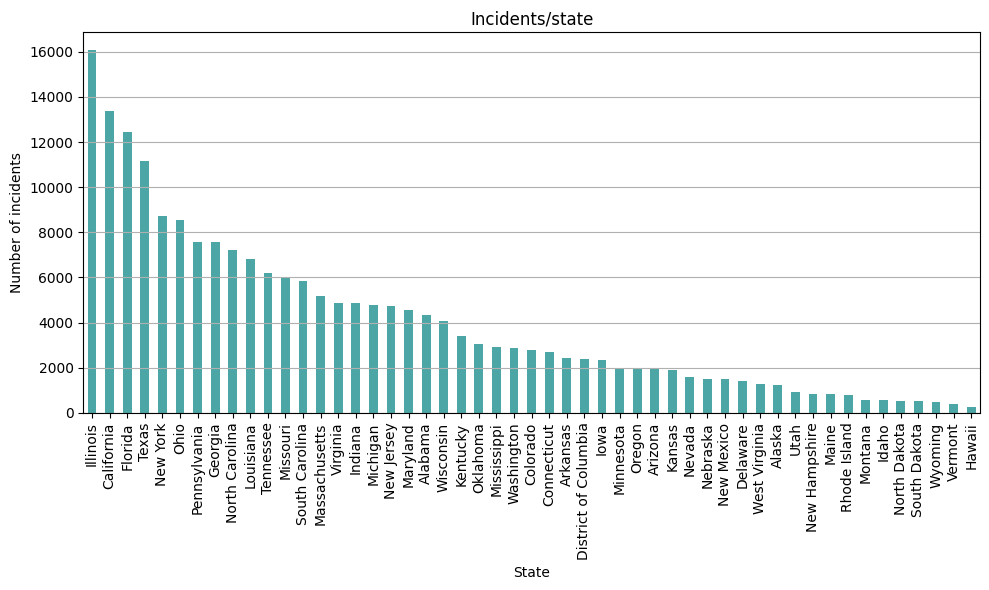
\includegraphics[width=0.8\textwidth]{incidents_per_state}
	\centering
	\caption{Number of incidents per state.}
	\label{incidents_per_state}
\end{figure}

The \textit{city\_or\_county} attribute has no null values, but it often contains additional informations about the suburb or the neighborhood in brackets, that provide a more precise location for the incident, e.g. ``Minneapolis (Brooklyn Center)".
We consider removing this kind of information in the next phase.
There are also instances containing the substring ``(county)" at the end, e.g. ``Orange (county)", that also appears as ``Orange": these instances will be substituted using just the name of the city/county.
Figure \ref{incidents_per_citycounty} shows the number of incidents recorded in each city/county in decreasing order.
\begin{figure}[H]
	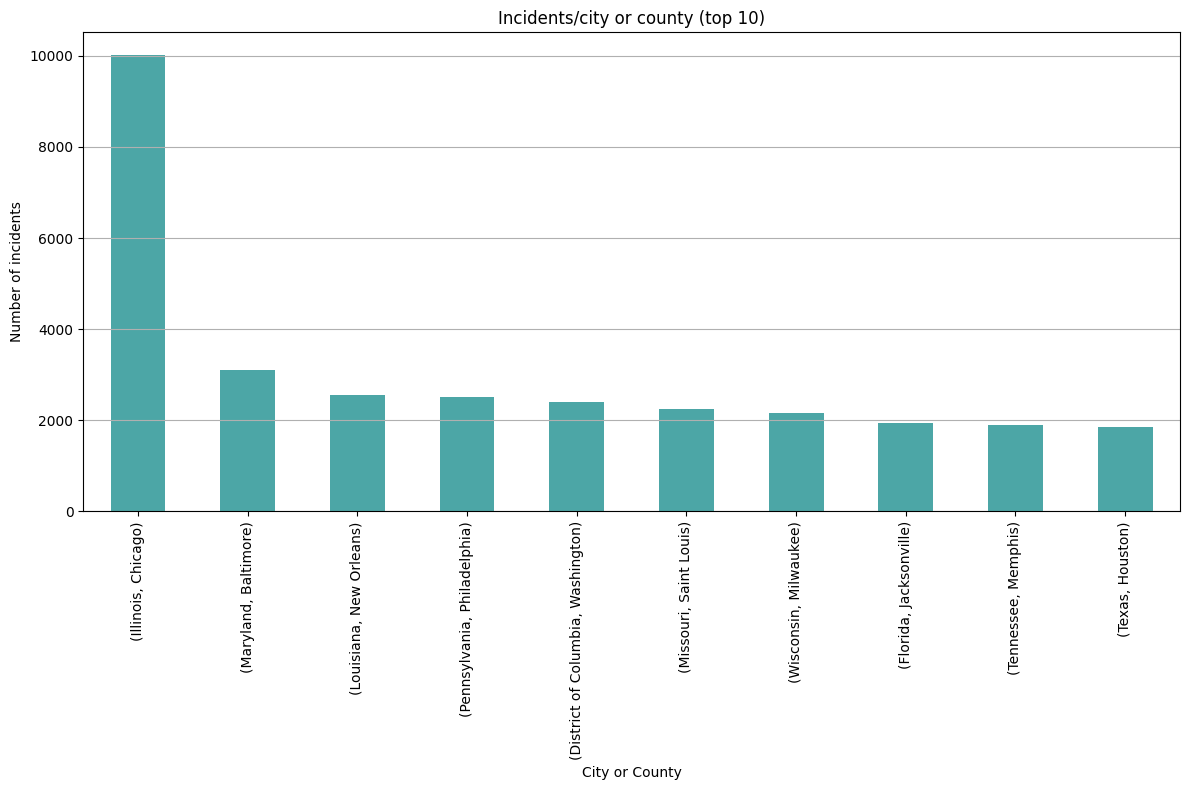
\includegraphics[width=0.8\textwidth]{incidents_per_citycounty}
	\centering
	\caption{Number of incidents per city or county.}
	\label{incidents_per_citycounty}
\end{figure}

The \textit{address} attribute contains some null values, but we believe it does not hold any statistical value, given that more specific information about the exact location of an incident is found by using the geographical coordinates.
Furthermore, there are only 6020 records for which address information can not be inferred using \textit{latitude} and \textit{longitude} attributes, so we will remove this column.

The \textit{latitude} and \textit{longitude} attributes contain some null values.
We also noticed some outliers by drawing empirical box boundaries of the United States: there are some incidents recorded outside of the U.S. that will be removed in the next phase.

Attributes \textit{congressional\_district}, \textit{state\_house\_district} and \textit{state\_senate\_district} contain some null values.
We also noticed that most of the incidents happened in the state of Illinois, by plotting the top 10 incidents for each of these attributes.

\subsubsection{Age and gender information}

The \textit{participant\_age1} attribute contains some outliers, mostly being values of type string and values that are too large to be the age of a person.
There are also some outliers if this attribute is compared to the corresponding value reported in the \textit{participant\_age\_group1} field.
As shown in Figure \ref{incidents_per_agegender}, most of the participants are adult males.
The attributes \textit{participant\_age1}, \textit{min\_age\_participants}, \textit{max\_age\_participants} and \textit{avg\_age\_participants} all have similar distributions.

The attributes \textit{n\_participants\_child}, \textit{n\_participants\_teen} and \textit{n\_participants\_adult} all present the same issues: they all contain outliers given by non-numerical strings, very large or negative numbers.

\begin{figure}[H]
	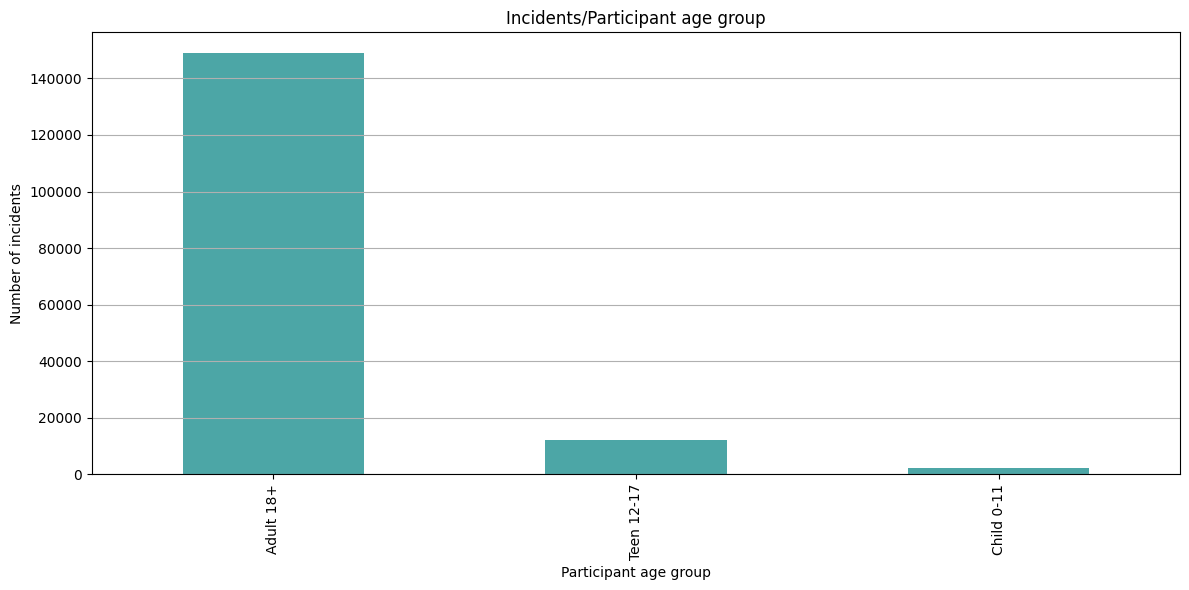
\includegraphics[width=0.8\textwidth]{incidents_per_agegroup}
	\centering
	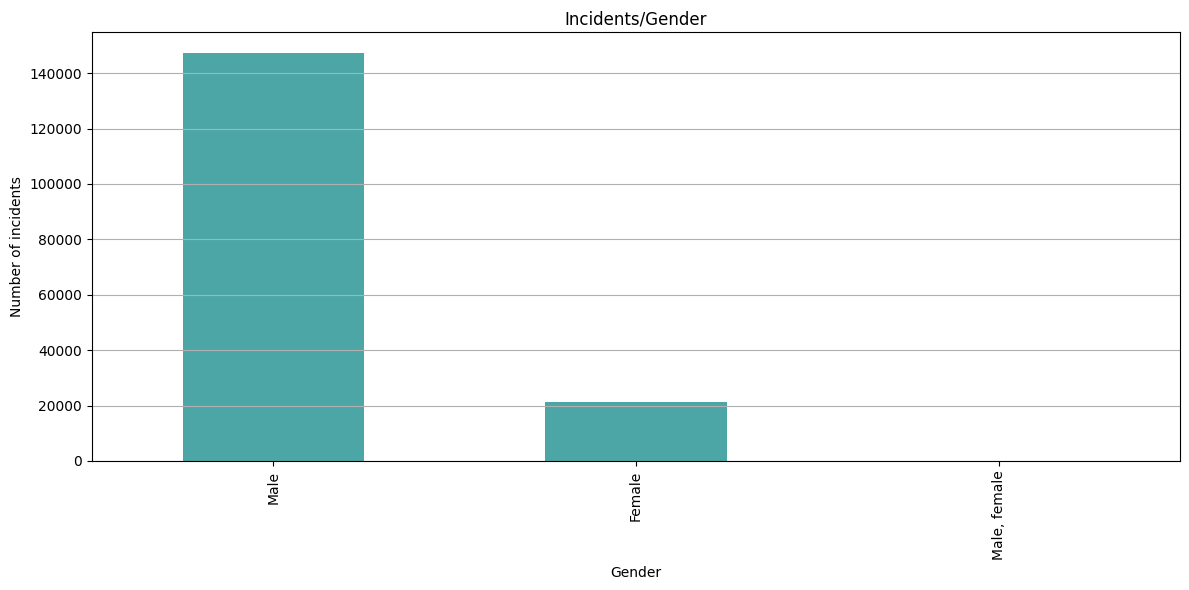
\includegraphics[width=0.8\textwidth]{incidents_per_gender}
	\caption{Number of incidents per age group (above) and gender (below) of the randomly chosen participant.}
	\label{incidents_per_agegender}
\end{figure}

\subsubsection{Number of involved people}

The majority of the incidents only involve between 0 and 5 people, with almost no killed, injured, unharmed or arrested people.

\subsubsection{Notes and incident characteristics}

We consider these attributes to hold no statistical value.

\subsection{Poverty by state}

The \textit{state} attribute contains 52 unique values: 51 of them are the same as the states in the incidents dataset, the remaining one is labeled ``United States" and contains the average of the whole country.
We consider using the average to possibly fill the missing values in the following phase.

There are no \textit{povertyPercentage} values for the year 2012, but we are only interested in relating this information to the incidents dataset, which only contains relevant incidents in the range of years 2013-2018.

\subsection{Year state district house}

This dataset contains no null values.
We will only consider data in the range of years 2013-2018 for integrating this data with the incidents dataset.

\section{Data Integration}

We created an additional column called \textit{total\_votes\_for\_state} in the year-state-house-district dataset: this column contains the total number of votes for each state and for each year.
We merged the incidents dataset with the poverty dataset using the attributes \textit{state} and \textit{year}.
We then merged the resulting dataset with the remaining one using the attributes \textit{state}, \textit{year} and \textit{congressional\_district}.
During the data integration process, records containing incidents set outside the U.S. were automatically deleted, resulting in a dataset that has no outliers in attributes \textit{latitude} and \textit{longitude}.
The dataset obtained by data integration will be used to further analyze and relate political party and poverty percentage to each congressional district.

\section{Distribution Analysis}

In order to analyze the features in the dataset, we displayed and examined the distribution of each column.
Figure \ref{age_du} shows the plots related to age attributes: as previously said, they all have very similar distributions.

\begin{figure}[h]
	\centering
	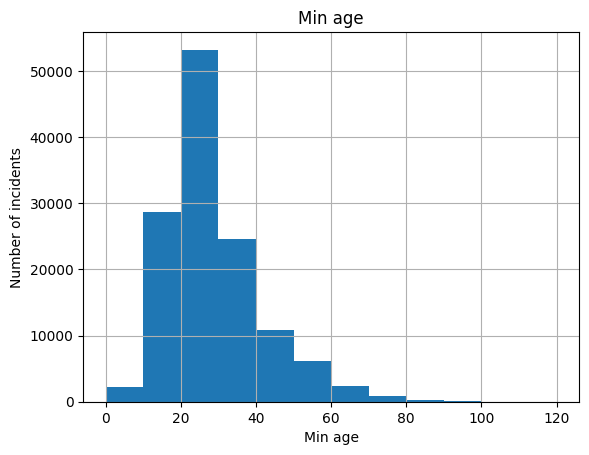
\includegraphics[width=0.5\textwidth]{min_age_du}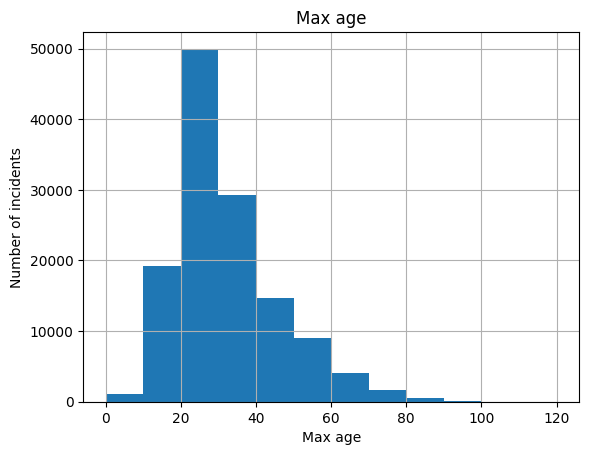
\includegraphics[width=0.5\textwidth]{max_age_du}
	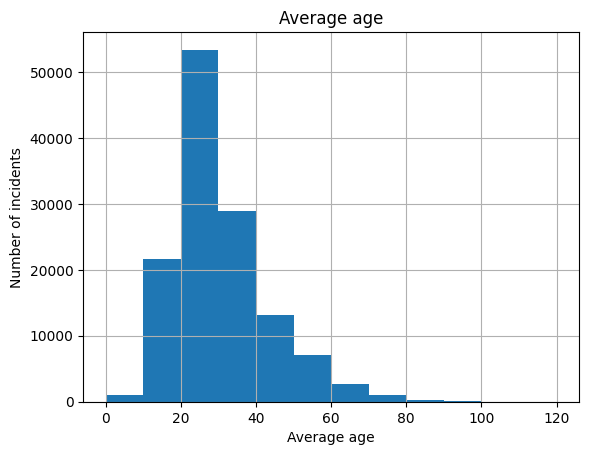
\includegraphics[width=0.5\textwidth]{avg_age_du}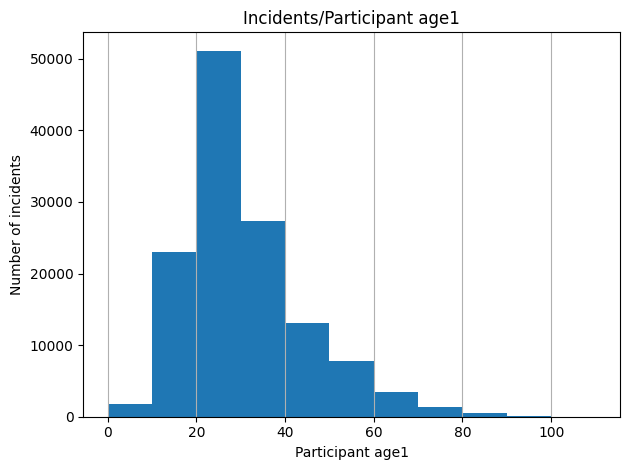
\includegraphics[width=0.5\textwidth]{part_age_du}
	\caption{Plot of minimum (top left), maximum (top right), average (bottom left) and participant1 (bottom right) age distributions.}
	\label{age_du}
\end{figure}

From Figure \ref{incidents_per_nparticipants} we can see that most of the incidents involve very few participants.
Specifically, the majority of them only involve between 0 and 3 participants, with incidents having only one person involved being the most common ones.

\begin{figure}[h]
	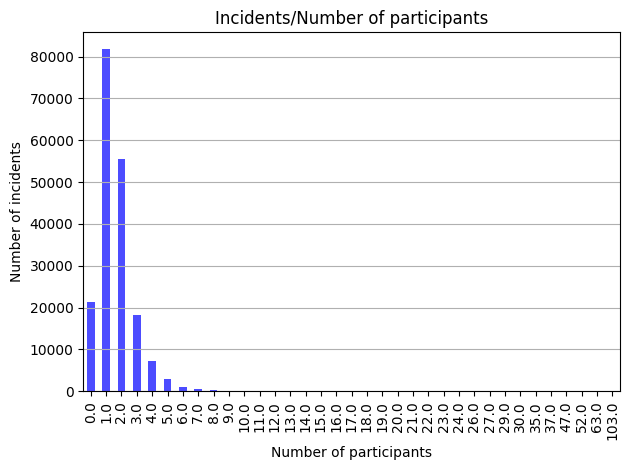
\includegraphics[width=0.7\textwidth]{incidents_per_nparticipants}
	\centering
	\caption{Number of incidents per number of people involved.}
	\label{incidents_per_nparticipants}
\end{figure}

As previously shown in Figure \ref{incidents_per_agegender}, the majority of participants recorded in the incidents is comprised of adult (18 years old or older) and male people.

\textbf{TODO} \textit{aggiungere gli screen dei plot delle mappe, quella degli shooting e quella dei mass shooting. in questo momento però non riesco a fare gli screen}\\
We also analyzed the geographical distribution of the incidents over the U.S. territory.
Specifically we focused on the number of killed people in each incidents in order to possibly understand the relation between killed people and geographical location.
The plots in Figure \ref{map_du} show the individual incidents recorded and the mass shooting events.
The incidents that resulted in 0 to 5 killed people are the majority, so the first map does not hold much meaning, given that most of the dots are records that report no killed people.
The second plot instead highlights events that are to be considered mass shootings and it shows some major events like, for example, Orlando (Florida) mass shooting in 2016 (50 killed people) and Southerland Springs (Texas) mass shooting (27 killed people).

\begin{figure}[h]
	\centering
	% TODO
	%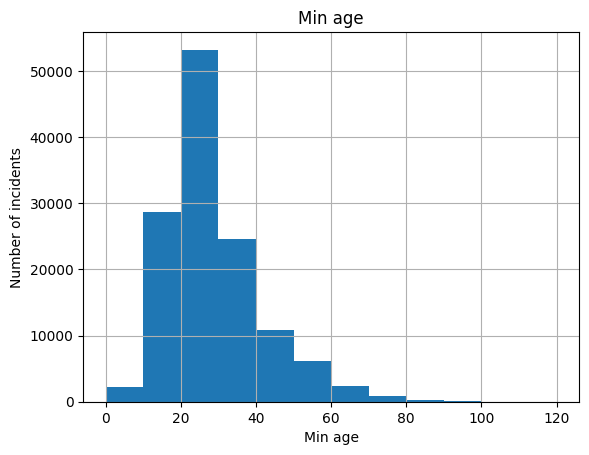
\includegraphics[width=0.5\textwidth]{min_age_du}\includegraphics[width=0.5\textwidth]{map_shooting}
	%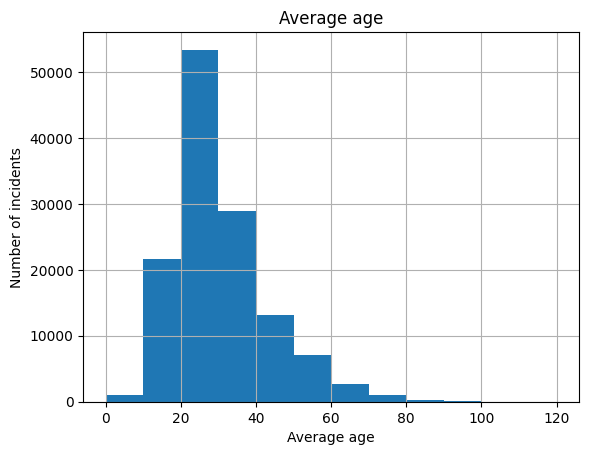
\includegraphics[width=0.5\textwidth]{avg_age_du}\includegraphics[width=0.5\textwidth]{map_massshooting}
	\caption{Map representing each incident (left) and mass-shooting incidents (right) recorded, the color used for the representation varies in relation to the number of people killed in the incident.
	The FBI has not set a minimum number of casualties to qualify an event as a mass shooting, but U.S. statute (the Investigative Assistance for Violent Crimes Act of 2012) defines a ``mass killing" as ``3 or more killings in a single incident." (\href{https://www.britannica.com/topic/mass-shooting}{source})}
	\label{map_du}
\end{figure}

\section{Correlation Analysis}

The correlation matrix is shown in Figure \ref{corr_matrix_du}.
At first glance, the only noteworthy correlations are those between the \textit{participant\_age1} feature of the randomly taken person and the attributes \textit{min\_age\_participants}, \textit{max\_age\_participants} and \textit{age\_age\_participants}.
This correlation is confirmed by the fact that the majority of the incidents only involve 1 or 2 participants. 
The correlation matrix will be computed again once outliers in the numerical attributes, which compromise the correlation calculation, have been eliminated.

We also observed that the number of males involved has a high correlation (0.83) with the number of participants because on average, as seen above, incidents tend to have a much more higher number of males participants than females participants.

\begin{figure}[h]
	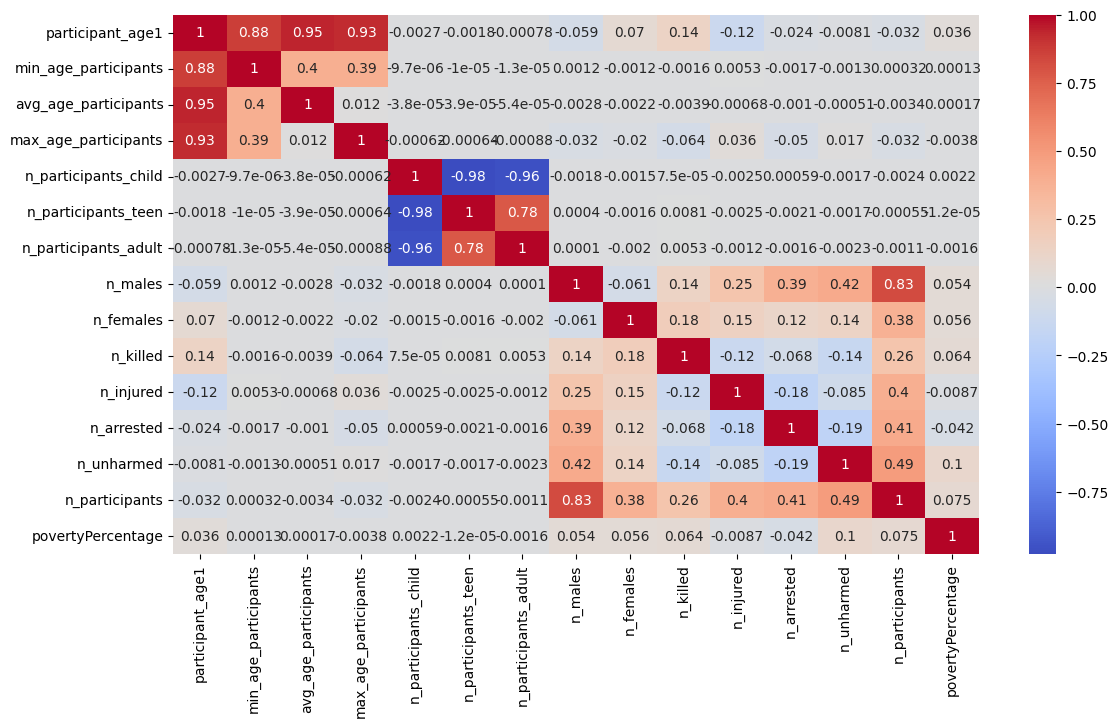
\includegraphics[width=1\textwidth]{corr_matrix_du}
	\centering
	\caption{Correlation matrix of numerical attributes.}
	\label{corr_matrix_du}
\end{figure}


\chapter{Data Preparation}

The data preparation phase uses the information gained in the previous phase to select records, manage outliers and missing values and improve data quality.
We started by changing the data types of the attributes as shown in Table \ref{table01}.

\begin{table}
	\centering
	\begin{small}
	\begin{tabular}{|l|l|l|p{7cm}|}
		\hline
		\textbf{Feature Name} & \textbf{Initial Type} & \textbf{Cast Type} & \textbf{Description}\\
		\hline
		date & object & Datetime64 & date of incident occurrence\\
		\hline
		state & object & String & state where incident took place\\
		\hline
		city\_or\_county & object & String & city or county where incident took place\\
		\hline
		address & object & String & address where incident took place\\
		\hline
		latitude & float64 & float64 & latitude of the incident\\
		\hline
		longitude & float64 & float64 & longitude of the incident\\
		\hline
		congressional\_district & int64 & Int64 & congressional district where the incident took place\\
		\hline
		state\_house\_district & int64 & Int64 & state house district\\
		\hline
		state\_senate\_district & float64 & Int64 & state senate district where the incident took place\\
		\hline
		participant\_age1 & float64 & Int64 & exact age of one (randomly chosen) participant in the incident\\
		\hline
		participant\_age\_group1 & object & String & exact age group of one (randomly chosen) participant in the incident\\
		\hline
		participant\_gender1 & object & String & exact gender of one (randomly chosen) participant in the incident\\
		\hline
		min\_age\_participants & object & Int64 & minimum age of the participants in the incident\\
		\hline
		avg\_age\_participants & object & float64 & average age of the participants in the incident\\
		\hline
		max\_age\_participants & object & Int64 & maximum age of the participants in the incident\\
		\hline
		n\_participants\_child & object & Int64 & number of child participants 0-11\\
		\hline
		n\_participants\_teen & object & Int64 & number of teen participants 12-17\\
		\hline
		n\_participants\_adult & object & Int64 & number of adult participants (18 +)\\
		\hline
		n\_males & float64 & Int64 & number of males participants\\
		\hline
		n\_females & float64 & Int64 & number of females participants\\
		\hline
		n\_killed & int64 & Int64 & number of people killed\\
		\hline
		n\_injured & int64 & Int64 & number of people injured\\
		\hline
		n\_arrested & float64 & Int64 & number of arrested participants\\
		\hline
		n\_unharmed & float64 & Int64 & number of unharmed participants\\
		\hline
		n\_participants & float64 & Int64 & number of participants in the incident\\
		\hline
		notes & object & String & additional notes about the incident\\
		\hline
		incident\_characteristics1 & object & String & incident characteristics\\
		\hline
		incident\_characteristics2 & object & String & incident characteristics\\
		\hline
		year & int64 & Int64 & \\
		\hline
		povertyPercentage & float64 & float64 & poverty percentage for the corresponding state and year\\
		\hline
		party & object & String & winning party for the corresponding congressional\_district in the state, in the corresponding year\\
		\hline
		candidateVotes & int64 & Int64 & number of votes obtained by the winning party in the corresponding election\\
		\hline
		totalVotes & int64 & Int64 & total number of votes for the corresponding election\\
		\hline
		total\_votes\_for\_state & int64 & Int64 & total number of votes for each year and for each state\\
		\hline
	\end{tabular}
	\end{small}
	\caption{Features of the merged dataset}
	\label{table01}
\end{table}

We then removed negative values by setting them to NaN.

\subsubsection{Age attributes}

For the attributes \textit{participant\_age1}, \textit{min\_age\_participants}, \textit{max\_age\_participants} and \textit{avg\_age\_participants}, we considered values $\ge 120$ as outliers and we set them to NaN.
These three attributes seemed to be very correlated, so we consider deleting the columns \textit{min\_age\_participants} and \textit{max\_age\_participants} and only keeping \textit{avg\_age\_participants}.

\subsubsection{Date}

We considered all dates after 2023-10-01 (the date we received the dataset) to be outliers, in particular errors in the data.
We dropped all records related to year 2013, as the year was under-represented (only 242 records).

\subsubsection{Geographical attributes}

The records with coordinates outside U.S. (other that null values) were automatically deleted after the data integration.
We consider the triple \textit{$<$date,latitude,longitude$>$} to be a key identifying an incident: we assume that there are no incidents happening on the same day in the exact same geographic coordinates.
Hence, we decided to eliminate the records in which these 3 values are duplicate.

For the rows in which \textit{latitude} and \textit{longitude} are NaN, we filled the missing values using the mean computed for the respective \textit{state} and \textit{city\_or\_county}.

We decided to drop the columns \textit{state\_house\_district} and \textit{state\_senate\_district}, given that they represent further subdivisions of the US territory that are not pertinent to our analysis.
In fact, we are only interested in the \textit{congressional\_district}, because the electoral information has the same granularity.

\subsubsection{Number of participants' attributes}

We checked whether the number of killed, injured, arrested and unharmed people exceeded the total number of participants in that incident.
Since, \textit{n\_arrested} and \textit{n\_killed} were the only two attributes with null values, we set them to 0 in case \textit{n\_participants} was 0; we filled the remaining null values using the mean.

We set to NaN the outliers found in \textit{n\_participants\_adult}, \textit{n\_participants\_teen} and \textit{n\_participants\_child} found during data understanding.
The outliers considered in this step were the values larger than the maximum values of \textit{n\_participants}.
We also set to zero the attributes \textit{n\_participants\_adult}, \textit{n\_participants\_teen}, \textit{n\_participants\_child}, \textit{n\_males} and \textit{n\_females} when \textit{n\_participants} is 0.
We replace the value in \textit{n\_participants} with the sum \textit{n\_males} + \textit{n\_females}, if this sum is equal to (\textit{n\_participants\_adult} + \textit{n\_participants\_teen} + \textit{n\_participants\_child}) and different from \textit{n\_participants}.
Viceversa, we set to NaN these attributes in the rows where the sums and/or \textit{n\_participants} are not equal.
We then substituted NaN values using the mean of each attribute and dropped the few rows for which we were not able to reconstruct the mean.

\subsubsection{Incident characteristics}

We dropped the column \textit{incident\_characteristics2} given that it has 40\% of null values and does not add meaningful details for our analysis.

\section{Correlation analysis}

We plotted the correlation matrix (Figure \ref{corr_matrix}) only for the numerical attributes.
We noticed that age attributes are highly correlated: we decided to drop all of them\footnote{We dropped \textit{participant\_age1}, \textit{min\_age\_participants} and \textit{max\_age\_participants}.} except for \textit{avg\_age\_participants}, which is the most correlated to the other attributes and gives us more general informations about all the participants.
Given the fact that we dropped \textit{participant\_age1}, then the attributes \textit{participant\_gender1} and \textit{participant\_age\_group1} become useless, so we dropped them.
To fill NaN values in \textit{avg\_age\_participants} we used the mean of each grouping on \textit{n\_participants}.

\begin{figure}[h]
	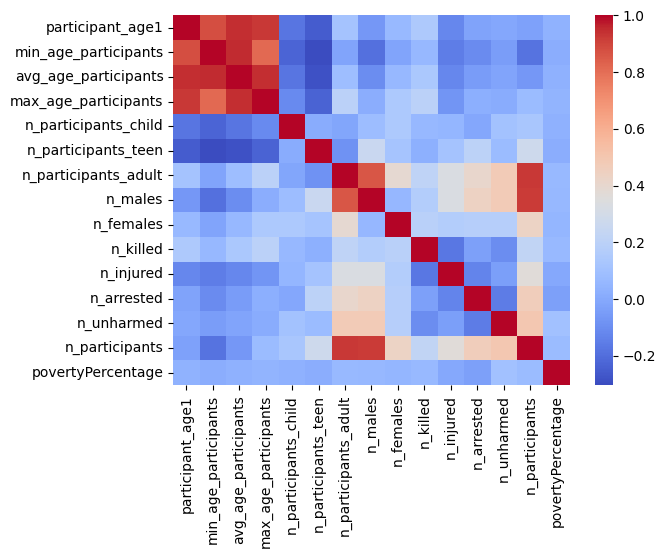
\includegraphics[width=0.8\textwidth]{corr_matrix}
	\centering
	\caption{Correlation matrix plotted of the numerical attributes}
	\label{corr_matrix}
\end{figure}

\section{Definition of indicators}

We computed the following indicators:
\begin{itemize}
	\item \textit{males\_percentage\_per\_city} (\textit{females\_percentage\_per\_city}), the number of males (females) involved in an incident over the total number of males (females) involved in incidents in the same city over the same time period;
	\item \textit{killed\_percentage\_per\_district} (\textit{injured\_percentage\_per\_district}, \textit{arrested\_percentage\_per\_district}, \textit{unhar\-med\_percentage\_per\_district}), the number of killed (injured, arrested, unharmed) people in an incident over the total number of people killed (injured, arrested, unharmed) in incidents in that same congressional district over the same time period;
	\item \textit{killed\_percentage\_per\_incident}, the number of killed people in each incident over the total number of participants in that same incident;
	\item \textit{unharmed\_percentage}, the number of unharmed people in the incident over the average of unharmed people in all the incidents in the same time period;
	\item \textit{arrest\_percentage}, the number of arrested people over the total number of participants in each incident;
	\item \textit{killed\_rate\_per\_state} (\textit{injured\_rate\_per\_state}, \textit{arrested\_rate\_per\_state}, \textit{unharmed\_rate\_per\_state}), the total number of people killed (injured, arrested, unharmed) per date and state over the total number of people killed (injured, arrested, unharmed) in that same date;
	\item \textit{age\_entropy\_per\_state}, the entropy of the \textit{avg\_age\_participants} grouped for date and state;
	\item \textit{winning\_party\_percentage}, the number of votes of the winning candidate over the total number of votes for that election.
\end{itemize}

We then plotted the correlation matrix (Figure \ref{corr_matrix_indicators}) for the indicators defined above.

\begin{figure}[h]
	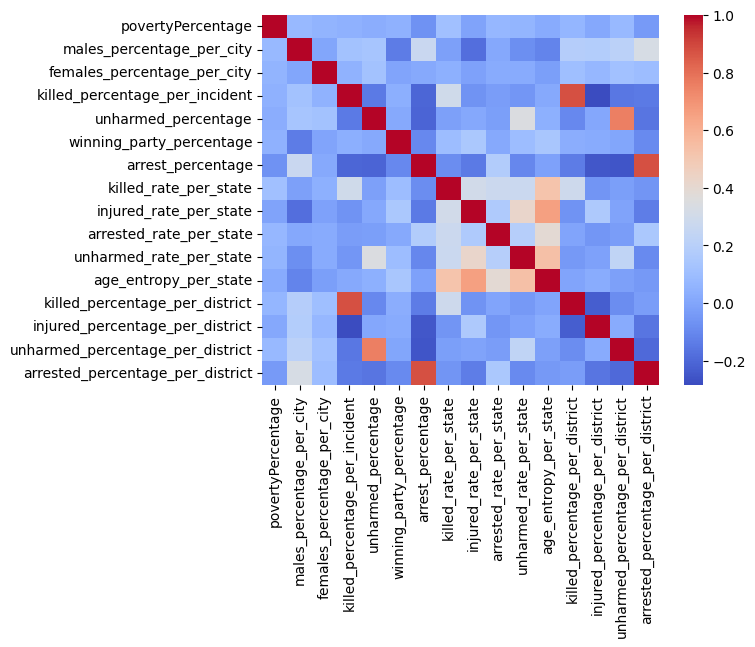
\includegraphics[width=0.8\textwidth]{corr_matrix_indicators}
	\centering
	\caption{Correlation matrix plotted of the newly created indicators}
	\label{corr_matrix_indicators}
\end{figure}

We also decided to drop the columns \textit{year} (just a result of data integration), \textit{address} and \textit{notes}.

\chapter{Clustering}

In order to prepare data for applying the clustering algorithms, we did some steps of preprocessing.
First of all we added a binary column \textit{involve\_killing} that has value 0 nobody was killed in the incident, and it has value 1 if there was at least a person killed in the incident.
We applied a normalization to numerical values.
The we computed the PCA with 2 components and got the visualization showed in Figure \ref{pca}.

\begin{figure}[h]
	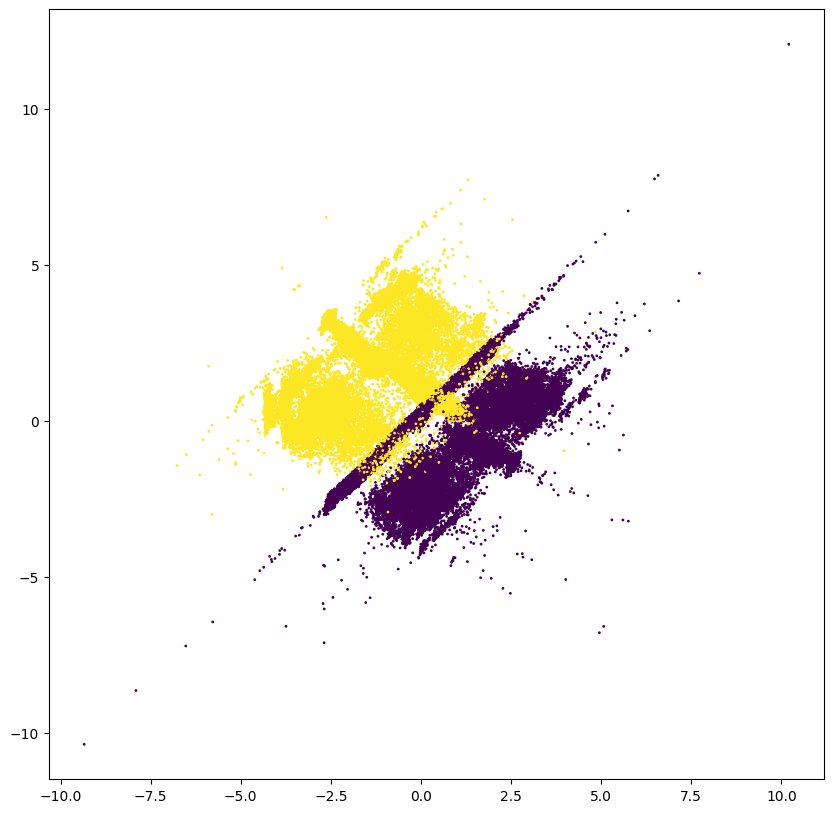
\includegraphics[width=0.8\textwidth]{pca}
	\centering
	\caption{Principal component analysis, computed on 2 components.
	The color of the points corresponds to the value of \textit{involve\_killed}.}
	\label{pca}
\end{figure}

\section{K-Means}

\subsection{X-Means}

\section{Hierarchical clustering}

\section{Dbscan clustering}

\end{document}
